\documentclass{article}
\usepackage[utf8x]{inputenc}
\usepackage[english,russian]{babel}
\usepackage{graphicx}
\usepackage{hyperref}
\begin{document}
\title{Тестирование алгоритма миграции Кирхгофа на слоистой модели из ПО Madagascar}
\author{\textbf{м.н.с. Голубев В.И.} \\ Лаборатория прикладной вычислительной геофизики МФТИ}
\maketitle

В Интернете нашёл комплекс Madagascar для обработки геофизической информации.
С его помощью (изменив немного примеры) получилось сгенерировать сейсмограмму (zero-offset) для слоистой среды.
При этом скоростная модель $C_p=2000$ м/с, а отражателями выступают границы раздела (см. рис. \ref{img_model}).

\begin{figure}[ht]
  \center
  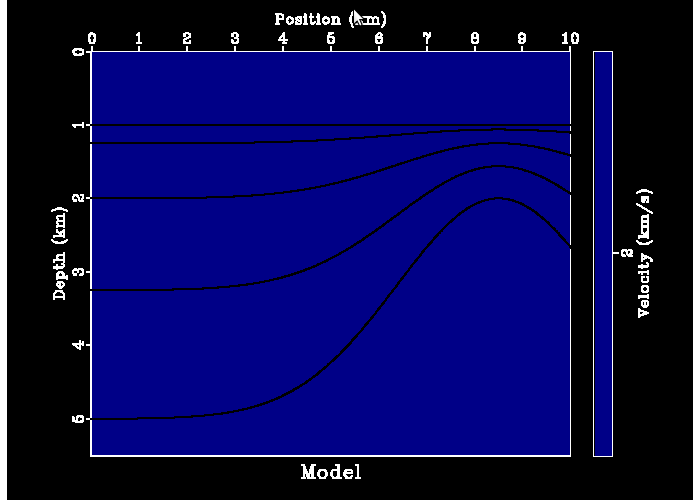
\includegraphics[scale=0.5]{pic/model.png}
  \caption{Модель среды с криволинейными границами. $C_p=2000$ м/с. Отражатели - границы раздела.}
\label{img_model}
\end{figure}

Madagascar имеет функцию вычисления zero-offset сейсмограммы методом Кирхгофа.
Она приведена на рис. (\ref{img_madagascar_input}).

\begin{figure}[ht]
  \center
  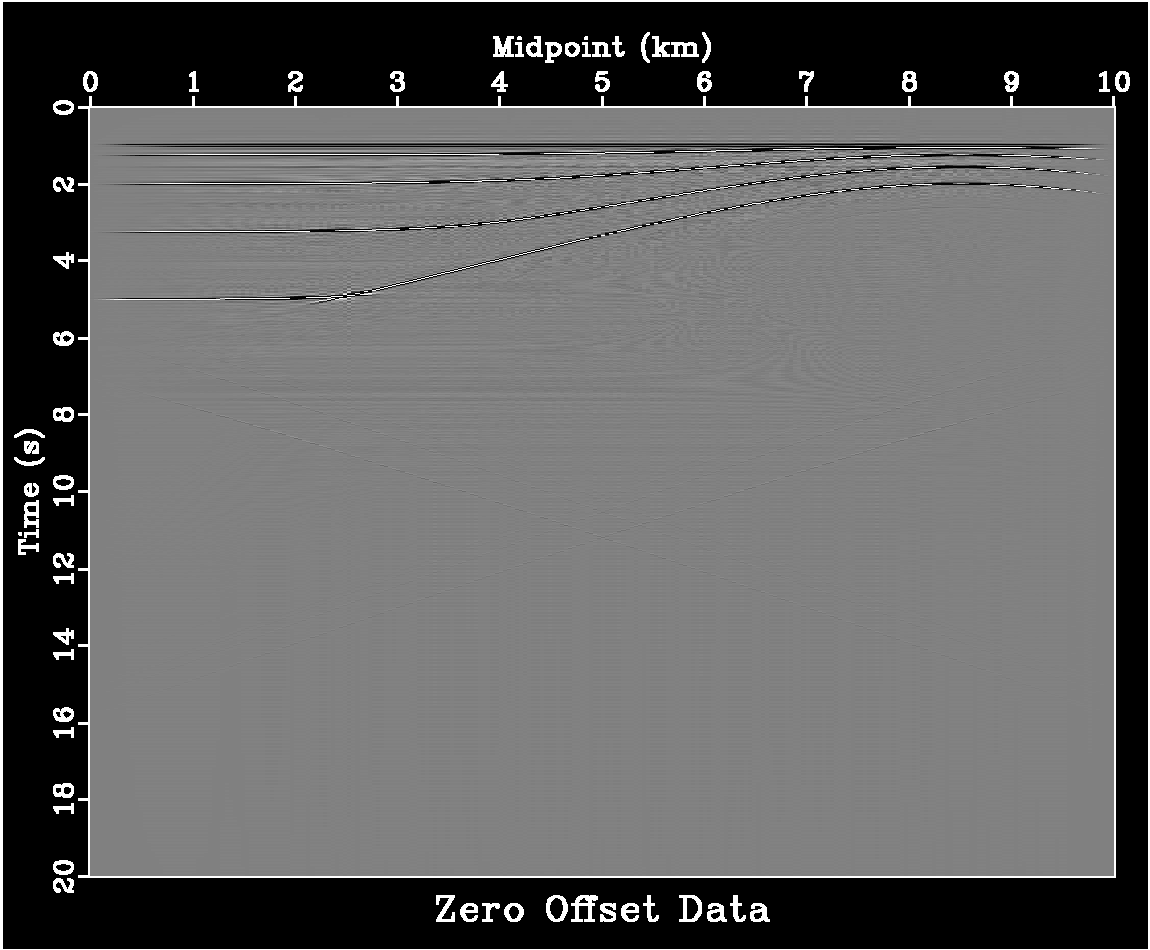
\includegraphics[scale=0.3]{pic/madagascar_input.png}
  \caption{Синтетическая сейсмограмма, построенная в Madagascar.}
\label{img_madagascar_input}
\end{figure}

При этом в Madagacar также можно сделать инверсию (какие-то усовершенствованные методы Кирхгофа) и получить отражающие границы (см. рис. \ref{img_madagascar_inverted}).

\begin{figure}[ht]
  \center
  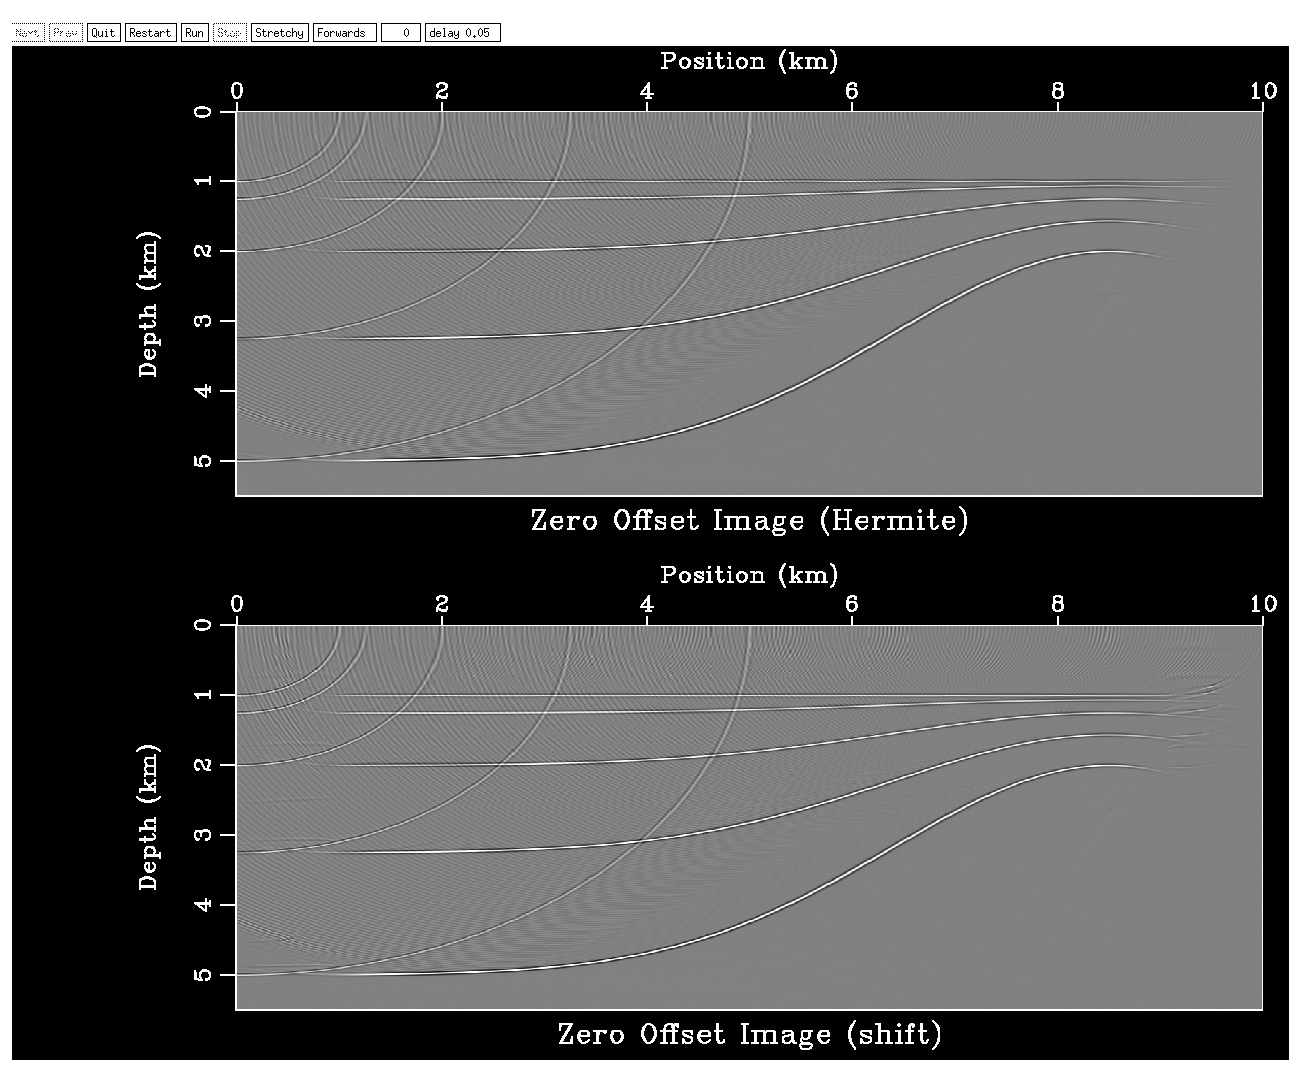
\includegraphics[scale=0.3]{pic/madagascar_inverted.png}
  \caption{Изображение после инверсии в Madagascar.}
\label{img_madagascar_inverted}
\end{figure}

Я дописал к своему AcInverse чтение из формата сейсмограммы Madagascar и просто запустил реализованную ранее процедуру миграции Кирхгофа.
На рис. \ref{img_acinverse_inverted} представлено получившееся изображение.
Видно, что процедура нашей миграции работает.

Как я и предполагал, вся проблема была в том, что входные данные должны быть специальным образом подготовлены.
Очень хотелось бы подробнее понять, какая именно обработка выполняется.
Тогда можно будет в нашем комплексе rect её реализовать и попробовать к его результатам применить инверсию.

\begin{figure}[ht]
  \center
  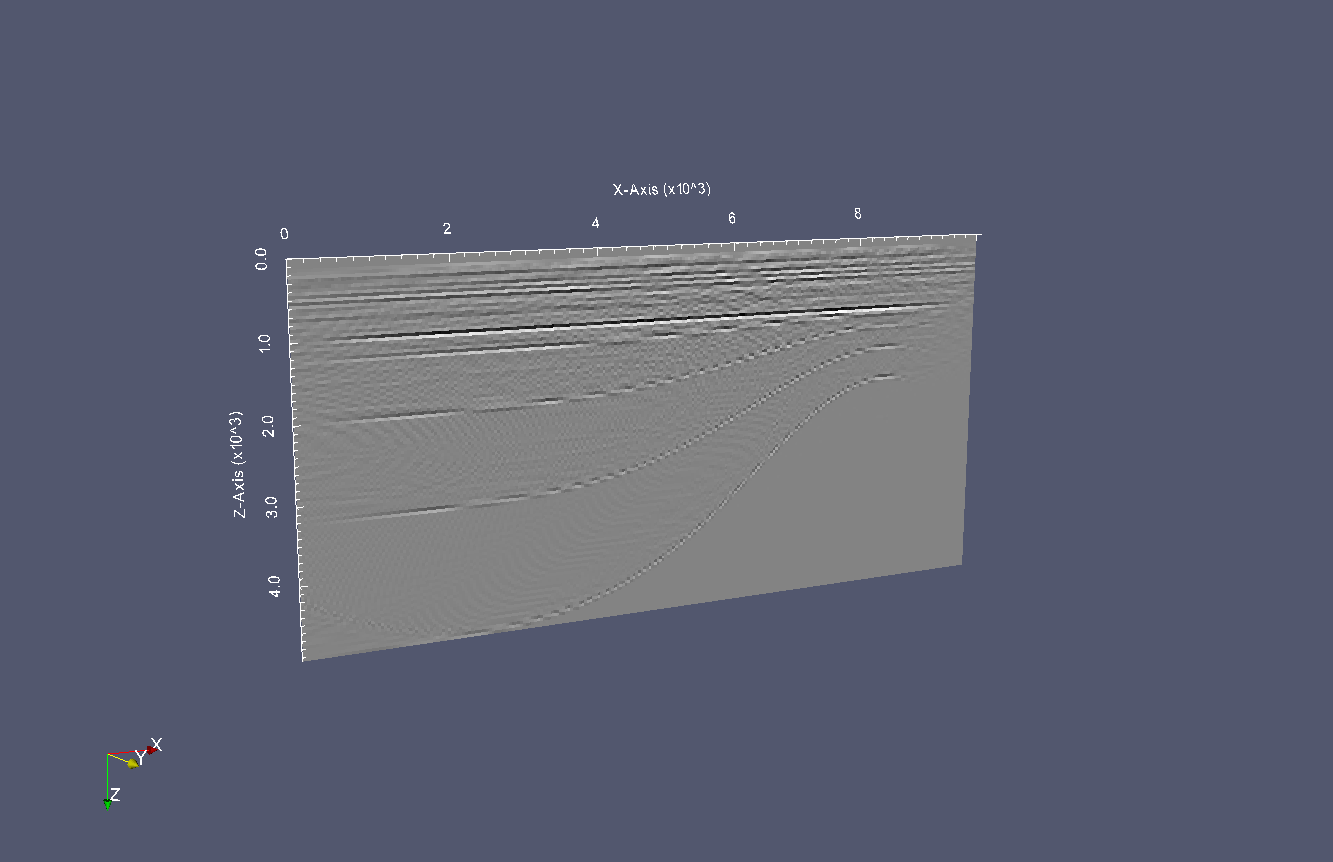
\includegraphics[scale=0.3]{pic/acinverse_inverted.png}
  \caption{Изображение после наешй инверсии в AcInverse.}
\label{img_acinverse_inverted}
\end{figure}

\end{document}
